\chapter{Symmetric-key Cryptography} % Main chapter title
\label{Symmetric-key Cryptography} % For referencing the chapter elsewhere, use \ref{Chapter1} 

\textit{Symmetric-key} cryptography (also commonly referred to as \textit{private-key cryptography}) is a system of cryptography which
uses the same keys for both encryption of plaintext and decryption of ciphertext. The keys must be shared between the different
parties accessing and handling the information. The requirement that all (authorized) parties must have access to the secret key
is the biggest drawback of symmetric-key cryptography \cite{wiki:symmetric_key_cryptography}.     

This chapter will discuss and implement the different types of symmetric-key cryptography algorithms. 
First we will explore and implement the various classical cryptography examples (some of which are discussed in the 
\hyperref[Early Cryptography]{Early Cryptography} chapter). From there, we will continue and take a look at more complex modern-day algorithms 
and discuss their implementation. 

\section{Transposition Ciphers}

One of the simplest methods of cryptography, a transposition cipher, works by changing the ordering of the message to make it seemingly unreadable.
This is similar to an anagram but with a regular defined structure to make it easily decryptable (assuming you know the defined structure or the \textit{key}).   

Mathematically, the ciphertext will be a permutation of the original plaintext. We can use an encryption function to encrypt our plaintext and then use 
the \textit{inverse} of our encryption function to decrypt our ciphertext. A generic transposition cipher (one with no specific encryption function) 
can be expressed mathematically as follows: $$\mathlarger{P \rightarrow E, f(x)}$$

In this example, we are mapping the set $P$ containing the plaintext to the set $E$ containing the ciphertext using the encryption function $f(x)$. 
In mathematics, this would be referred to a \textit{bijection} from set $P$ to $E$. Keep in mind that while transposition ciphers certainly
are functions, we can not easily assign them a simple algebraic formula since they deal with the positions of letters rather than the letters themselves.

Decryption of the ciphertext is defined in a similar fashion, but instead we use the \textit{inverse bijection} from our ciphertext set $E$ to $P$. 
Notice that now our function $f(x)$ is inversed becoming: $f^{-1}(x)$. The algebraic expression for decryption is written as follows: 
$$\mathlarger{E \rightarrow P, f^{-1}(x)}$$

Though there are many different types of transposition ciphers, in this section we will only discuss one and it's benefits, drawbacks, and efficiency.

\subsection{Rail Fence Cipher}

The \textit{rail fence cipher} (also referred to as a \textit{ZigZag} cipher) is a form of transposition cipher which arranges letters from
the plaintext in different "rails." It works by writing letters downwards and diagonally on following "rails" of an 
\textit{imaginary fence} (hence where the name of this cipher comes from). When we reach the bottom rail, we begin writing 
letters upwards. Likewise, when we reach the top rail, we begin writing letters downwards again until the whole plaintext is
written on our rail fence. For instance, if our fence has \textit{3} rails and our plaintext is:
'\textit{WE ARE DISCOVERED FLEE AT ONCE}', the ciphertext would look like so:

\begin{listing}[H]
    \begin{minted}[mathescape,
        numbersep=5pt,
        frame=lines,
        framesep=2mm]{text}
    
W . . . E . . . C . . . R . . . L . . . T . . . E
. E . R . D . S . O . E . E . F . E . A . O . C .
. . A . . . I . . . V . . . D . . . E . . . N . .
    
    \end{minted}
    \caption{Example of plaintext encrypted using the rail fence cipher. In this example, we have removed
    all whitespaces in the plaintext.}
\end{listing}

This is then read off to get the ciphertext:

\begin{minted}[mathescape,
    numbersep=5pt,
    frame=lines,
    framesep=2mm]{text}
    
WECRL TEERD SOEEF EAOCA IVDEN
\end{minted}

Decryption is done in a similar fashion by laying out the ciphertext in appropriate rails. Let's take a look at how
you go about decrypting the ciphertext above. First, we must know the height and \textit{cycle} of the ciphertext. The height
is simply the amount of rails that was used to encrypt the plaintext. A cycle is the number of letters which run from the top 
row to the bottom row and then up again, but stops before the top-most row (where a new cycle begins). The cycle can be 
written mathematically as: $$\mathlarger{2R - 2}$$ 

This simply says that each cycle is double our number of rails, minus 2. This is because, when we double our number of rails
(for going up and down) we wil have a duplicate position at the bottom row, thus we subtract $1$. We then also 
subtract $1$ since our cycle does not include the top-most row. Do note that the rail index is \textit{zero based}. This means
that the \textit{first} rail will have an index of \textit{0} and the last rail will have an index of $n - 1$.

Next, we will need to know the distance between every character on a specific rail. If we refer back to our example,
you will notice that both the top and bottom rails have the \textit{same} spacing between each character. This is because,
both the top and bottom row are where cycles connect. If you think of it as a triangle, the vertices of the triangle are
layed out on the bottom and top rows. The equation for calculating the character distance is: $$\mathlarger{C - 2R}$$

In simple terms, we are getting the \textit{distance} between our cycle and our current rail (factoring both up and
 down movements). As previously mentioned, distance patterns alternate on middle rows, this alternation is our cycle
  minus our \textit{current} character distance. This can be written mathematically as follows: $$\mathlarger{D_n = C - D_c}$$

Where $C$ is our cycle, $D_c$ is our current character distance, and $D_n$ is our new character distance.

There is one last step to calculating the character distance: handling the bottom rail. The aforementioned distance equation
will \textit{not} work for the bottom rail. Instead, the character distance for the bottom rail is our cycle. 
In fact, the top rail is also the cycle but we don't need to manually handle that case as our equation does that for us 
(the subtraction is factored when the rail index is \textit{0}).

Given the cycle and character distance, we can simply reconstruct the rail fence by laying out the cipher
text according to the appropriate character distance. 

\begin{figure}[H]
    \centering
    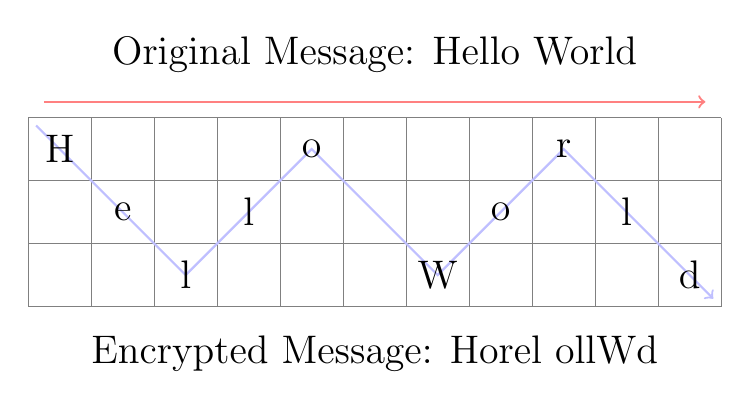
\begin{tikzpicture}
        \def\boxgap{+0.0cm}
        \def\minboxsz{0.8cm}
        \def\boxlinewidth{0.04cm}
        \def\stripgap{1cm}
        \def\lsgap{0.5cm}
         
        \node at(4.4, 3.2) {\Large Original Message: Hello World};
        \node at(4.4, -0.6) {\Large Encrypted Message: Horel ollWd};
        \draw[step=0.8cm,gray] (0,0) grid (11*\minboxsz,3*\minboxsz);
        \draw [->, thick, blue!25] (0.1, 2.3) -- (2.0, 0.4) -- (3.6, 2.0) -- (5.2, 0.4) -- (6.8, 2.0) -- (8.7, 0.1);
        \draw [->, thick, red!50] (0.2, 2.6) -- (8.6, 2.6);
        \node at(1*\minboxsz/2, 5*\minboxsz/2) {\Large H};
        \node at(3*\minboxsz/2, 3*\minboxsz/2) {\Large e};
        \node at(5*\minboxsz/2, 1*\minboxsz/2) {\Large l};
        \node at(7*\minboxsz/2, 3*\minboxsz/2) {\Large l};
        \node at(9*\minboxsz/2, 5*\minboxsz/2) {\Large o};
        \node at(13*\minboxsz/2, 1*\minboxsz/2) {\Large W};
        \node at(15*\minboxsz/2, 3*\minboxsz/2) {\Large o};
        \node at(17*\minboxsz/2, 5*\minboxsz/2) {\Large r};
        \node at(19*\minboxsz/2, 3*\minboxsz/2) {\Large l};
        \node at(21*\minboxsz/2, 1*\minboxsz/2) {\Large d};       
    \end{tikzpicture}
    \caption{A diagram of the rail fence cipher which demonstrates how plaintext is arranged on the rails.}
\end{figure}

Now that we have discussed the theory behind the Rail Fence cipher, we will go ahead and implement it.
First we will write the encryption function. To encrypt plaintext we need two key pieces of information:
our plaintext and the amount of rails to encrypt with. 

\begin{minted}[mathescape,
    numbersep=5pt,
    frame=lines,
    framesep=2mm]{python}
# Encryption function which takes in the plain_text and rail number.
def encrypt(plain_text, rails):
    # Create our cipher_text string and initialize to empty
    cipher_text = str()

    # TODO: Encryption

    return cipher_text
\end{minted}

As discussed previously, when encrypting, the message is laid out in rails according to the cycle. 
Therefore, we will need to calculate the cycle within our function. 
We can use the aforementioned equation to calculate the cycle. We use the \textit{max} function to 
make sure that our cycle stays above 1, it is simply a special case for an encryption with one rail.\footnote{Although 
encrypting plaintext with one rail won't yield particularly interesting results, we still make sure our algorithm can support it.}

\begin{minted}{python}
cycle = max(rails * 2 - 2, 1) # 1 is special case for 1 rail    
\end{minted}

Next we will write the letters of the plaintext to their corresponding position on the rail. 
We will iterate through every rail and layout characters which belong to that rail. 

In every iteration, we must calculate a few key pieces of data. First, we will need to know the distance between 
each character on the specific rail. As discussed, there is an alternating pattern between each character on a rail,
one for a character going down a cycle, and one for a character going up a cycle (with the top and bottom rails
having a constant spacing between characters). Since the top and bottom rails have the same spacing, if the rail
is the bottom rail, we set our distance to the cycle. Second, we will need to have a pointer variable which
keeps a reference to the current character we are looking at. This will simply be initialized to our rail (the start position
of the rail in the text). 

Laying out the letters is actually quite simply. Since we know the distance between each character, we can continue
iterating through the plaintext until our pointer is \textit{greater} than the length of our plaintext. In every iteration,
we increment the pointer by our character distance, making sure to alternate between the two distance patterns. 

Here is the iteration code along with the rest of the encryption function.

\begin{listing}[H]
    \begin{minted}[mathescape,
        numbersep=5pt,
        frame=lines,
        framesep=2mm]{python}
def encrypt(plain_text, rails):
    cipher_text = str()
    cycle = max((rails - 1) * 2, 1) # 1 is special case for 1 rail
            
    for rail in range(rails):
        ptr = rail
        character_distance = cycle - 2 * rail
                
        # Both the bottom and top rails have a (same) character distance of the cycle. 
        if rail == rails - 1:
            character_distance = cycle
        
        # While we have *something* to write
        while ptr < len(plain_text):
            cipher_text += plain_text[ptr]
            ptr += character_distance
        
            # If this is not the top or bottom rail 
            # alternate between two distance patterns
            if rail != 0 and rail != rails - 1:
                character_distance = cycle - character_distance
        
    return cipher_text
        \end{minted}
        \caption{Full implementation of encryption in the rail fence cipher.}
\end{listing}

The implementation for decryption is almost identical. Like encryption, when decrypting we must layout our ciphertext in the corresponding
rails. To do this, we can use the \textit{same} algorithm that we used for encryption. 

\begin{listing}[H]
    \begin{minted}[mathescape,
        numbersep=5pt,
        frame=lines,
        framesep=2mm]{python}
def decrypt(cipher_text, rails):
    plain_text = [''] * len(cipher_text)
    cipher_index = 0
    cycle = max((rails - 1) * 2, 1)  # 1 is special case for 1 rail
    
    for rail in range(rails):
        ptr = rail
        character_distance = cycle - 2 * rail
    
        # Both the bottom and top rails have a (same) character distance of the cycle. 
        if rail == rails - 1:
            character_distance = cycle
    
        # While we have *something* to write
        while ptr < len(plain_text):
            plain_text[ptr] = cipher_text[cipher_index]
            cipher_index += 1
                
            ptr += character_distance
            
            # If this is not the top or bottom rail
            # alternate between two distance patterns  
            if rail != 0 and rail != rails - 1:
                character_distance = cycle - character_distance
    
    return ''.join(plain_text)
        \end{minted}
        \caption{Full implementation of decryption in the rail fence cipher.}
\end{listing}

As you can see, there are only slight differences between the encryption and decryption implementations. The first difference is the
way we build our result text. When we \textit{encrypt}, we append characters to a string (which is our ciphertext). We can do this because
our ciphertext is \textit{one-dimensional}. Conversely, when we decrypt, since we are laying out characters on rails, we must preserve the order of the
fence; we can think of this as \textit{two-dimensional} (since we are not just laying out character horizontally). 
The second change, is the introduction of a second pointer variable: the \textit{cipher index}. 
This is simply used to track the current reading-index of the ciphertext (so we know what character to read next). 
There are some other \textit{small} changes in the decryption code but those are self-explanatory so they will not be covered.

\section{Substitution Ciphers}

A substitution cipher is a type of cryptography technique where each unit of plaintext is replaced with a unit of ciphertext; a unit may refer to a single
letter of the plaintext, a pair of letters, alternating patterns of the aforementioned, and so on \cite{wiki:substitution_cipher}.

A substitution cipher can be compared with a transposition cipher---the two are rather similar. In a transposition cipher, the units of plaintext are rearranged as a
permutation, but the units \textit{always} remained unchanged. The latter is unlike a substitution cipher which preserves the order of the plaintext but alters
the units.

\subsection{Caesar Cipher}
The Caesar Cipher, arguably the most popular form of substitution ciphers is another very simple form of cryptography. 
It works by replacing each letter by a certain number of letters up or down in the alphabet. The amount of 
letters that we move by is known as the \textit{shift offset}. If you shift the letter \textit{A} by 3 spaces, you get 
the letter \textit{D}. If you shift the letter \textit{B}, you get the letter \textit{E}.

% Caesar cipher diagram
\begin{figure}[H]
    \centering
    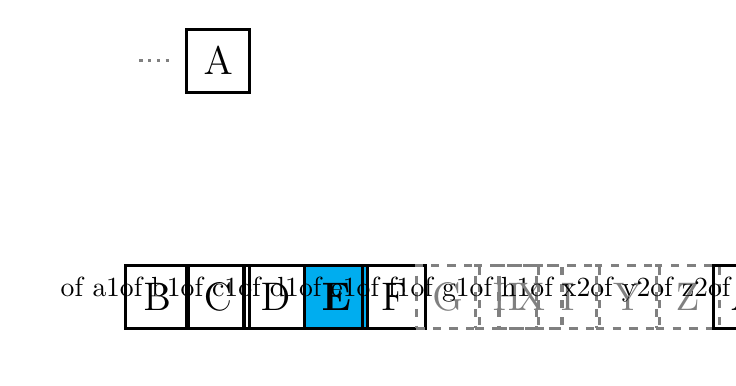
\begin{tikzpicture}
        \def\boxgap{+0.053cm}
        \def\minboxsz{0.8cm}
        \def\boxlinewidth{0.04cm}
         
        \draw[gray, dotted, line width=0.04cm] (1, 3) -- (1.4, 3);
        \node[rectangle, draw, line width=\boxlinewidth, minimum size=\minboxsz] (a1) at (2, 3) {\Large A};
        \node[rectangle, draw, line width=\boxlinewidth, minimum size=\minboxsz, right = \boxgap of a1] (b1) {\Large B};
        \node[rectangle, draw, line width=\boxlinewidth, minimum size=\minboxsz, right = \boxgap of b1] (c1) {\Large C};
        \node[rectangle, draw, line width=\boxlinewidth, minimum size=\minboxsz, right = \boxgap of c1] (d1) {\Large D};
        \node[rectangle, draw, line width=\boxlinewidth, minimum size=\minboxsz, right = \boxgap of d1, fill=cyan] (e1) {\Large \textbf{E}};
        \node[rectangle, draw, line width=\boxlinewidth, minimum size=\minboxsz, right = \boxgap of e1] (f1) {\Large F};
        \node[rectangle, draw, line width=\boxlinewidth, minimum size=\minboxsz, right = \boxgap of f1, dashed, gray] (g1) {\Large \textcolor{gray}{G}};
        \node[rectangle, draw, line width=\boxlinewidth, minimum size=\minboxsz, right = \boxgap of g1, dashed, gray] (h1) {\Large \textcolor{gray}{H}};
        \node[rectangle, draw, line width=\boxlinewidth, minimum size=\minboxsz, right = \boxgap of h1, dashed, gray] (i1) {\Large \textcolor{gray}{I}};
         
        \node[rectangle, draw, line width=\boxlinewidth, minimum size=\minboxsz, dashed, gray] (x2) at (0, 0) {\Large \textcolor{gray}{X}};
        \node[rectangle, draw, line width=\boxlinewidth, minimum size=\minboxsz, right = \boxgap of x2, dashed, gray] (y2) {\Large \textcolor{gray}{Y}};
        \node[rectangle, draw, line width=\boxlinewidth, minimum size=\minboxsz, right = \boxgap of y2, dashed, gray] (z2) {\Large \textcolor{gray}{Z}};
        \node[rectangle, draw, line width=\boxlinewidth, minimum size=\minboxsz, right = \boxgap of z2] (a2) {\Large A};
        \node[rectangle, draw, line width=\boxlinewidth, minimum size=\minboxsz, right = \boxgap of a2, fill=cyan] (b2) {\Large \textbf{B}};
        \node[rectangle, draw, line width=\boxlinewidth, minimum size=\minboxsz, right = \boxgap of b2] (c2) {\Large C};
        \node[rectangle, draw, line width=\boxlinewidth, minimum size=\minboxsz, right = \boxgap of c2] (d2) {\Large D};
        \node[rectangle, draw, line width=\boxlinewidth, minimum size=\minboxsz, right = \boxgap of d2] (e2) {\Large E};
        \node[rectangle, draw, line width=\boxlinewidth, minimum size=\minboxsz, right = \boxgap of e2] (f2) {\Large F};
        \draw[gray, dotted, line width=0.04cm] (7.8, 0) -- (8.2, 0);
         
        \draw [->, line width=0.04cm, gray] (a1) to[out=270, in=90] (x2);
        \draw [->, line width=0.04cm, gray] (b1) to[out=270, in=90] (y2);
        \draw [->, line width=0.04cm, gray] (c1) to[out=270, in=90] (z2);
        \draw [->, line width=0.04cm] (d1) to[out=270, in=90] (a2);
        \draw [->, line width=0.04cm] (e1) to[out=270, in=90] (b2);
        \draw [->, line width=0.04cm] (f1) to[out=270, in=90] (c2);
        \draw [->, line width=0.04cm, gray] (g1) to[out=270, in=90] (d2);
        \draw [->, line width=0.04cm, gray] (h1) to[out=270, in=90] (e2);
        \draw [->, line width=0.04cm, gray] (i1) to[out=270, in=90] (f2);
    \end{tikzpicture}
    \caption{A diagram of the Caesar cipher using a shift offset of \textit{3}.}
\end{figure}

Here is a simple example of a message encrypted using the cipher with a shift offset of 3:

\begin{minted}[mathescape,
               numbersep=5pt,
               frame=lines,
               framesep=2mm]{text}

Plaintext message: 
HELLO WORLD
               
Ciphertext message:
KHOOR ZRUOG
\end{minted}

Even though the ciphertext appears to be unreadable, substitution cipher remains to be one of the weakest forms of cryptography. 
This is for several reasons:
\begin{itemize}  
    \item The possible number of keys is very small, since the key is an offset by which to shift by, it is limited to the number of letters in the alphabet.
    In the case of the English alphabet, one could very easily try all 25 possibilities. 
    \item Since the structure of the original message remains intact, the ciphertext could be subjected to frequency-analysis which would reveal patterns about the message;
    potentially revealing the key.
    \item By studying multiple different ciphertexts, one could notice patterns within them and find out the key through that.
\end{itemize}

The substitution cipher can be expressed mathematically as follows: $$\mathlarger{E_i(n)=(n+k)\mod{26}}$$

Here we say that the encryption of the $ith$ letter $n$ is equal to a shift of $n+k$ where $k$ is the shift offset (or the key). The result of the shift
is divided by $26$ where the remainder of the division is used to make sure that the shift wraps around the alphabet; if the 
shift goes beyond the range of the alphabet ($0$ to $26$), it wraps around back to the beginning.

Decryption is done in a similar manner, but instead subtracting by $k$. $$\mathlarger{P_i(n)=(n-k)\mod{26}}$$

Please note that even though this example is for the English alphabet, the aforementioned equations should work for most languages assuming that they are modified
to the count of the specific languages' alphabet.

The concept of shifting letters is rather intuitive but how do we shift letters in code? This is done by representing
each letter as a \textit{number} and then \textit{adding} or \textit{subtracting} from this number by our shift
offset. The \textit{ASCII} (American Standard Code for Information Interchange) scheme is an encoding which 
provides the numerical representation of letters; this is known as an \textit{ordinal} \cite{caesar_cipher_invent_with_python}. 
We can use ASCII to implement this cipher. 

In the ASCII encoding scheme, the capital letters: \textit{A} through \textit{Z} are represented by the ordinals $65$ through 
$90$. The lowercase letters: \textit{a} through \textit{z} are represented by the ordinals $97$ through $122$. 
Lastly, the numeric digits $0$ through $9$ are represented by the ordinals $48$ through $57$.

Modern computers typically use the \textit{UTF-8} encoding instead of ASCII. Fortunately, UTF-8 is backwards compatible
with ASCII which means that the ordinals in UTF-8 will be the same as in ASCII.

The figure below shows the relevant parts of the ASCII table in all of it's glory!

\begin{table}[H]
    \centering
        \begin{tabular}{ | c c | c c | c c | c c | c c | c c |  } 
            \hline
            \multicolumn{12}{|c|}{ASCII Table} \\
            \hline
        % x & n     & x  & n & x  & n & x  & n & x  & n  & x   & n
            32 & (space) & 48 & 0 & 64 & @ & 80 & P & 96 & ` & 112 & p \\ 
            33 & !     & 49 & 1 & 65 & A & 81  & Q & 97  & a  & 113 & q \\
            34 & "  & 50 & 2 & 66 & B & 82 & R & 98 & b & 114 & r \\
            35 & \# & 51 & 3 & 67 & C & 83 & S & 99 & c & 115 & s \\
            36 & \$ & 52 & 4 & 68 & D & 84 & T & 100 & d & 116 & t \\
            37 & \% & 53 & 5 & 69 & E & 85 & U & 101 & e & 117 & u \\
            38 & \& & 54 & 6 & 70 & F & 86 & V & 102 & f & 118 & v \\
            39 & '  & 55 & 7 & 71 & G & 87 & W & 103 & g & 119 & w \\
            40 & (  & 56 & 8 & 72 & H & 88 & X & 104 & h & 120 & x \\
            41 & )  & 57 & 9 & 73 & I & 89 & Y & 105 & i & 121 & y \\
            42 & *  & 58 & : & 74 & J & 90 & Z & 106 & j & 122 & z \\
            43 & +  & 59 & ; & 75 & K & 91 & [ & 107 & k & 123 & \{ \\ 
            44 & ,  & 60 & < & 76 & L & 92 & \textbackslash & 108 & l & 124 & $\vert$ \\
            45 & -  & 61 & = & 77 & M & 93 & ] & 109 & m & 125 & \} \\
            46 & .  & 62 & > & 78 & N & 84 & \textasciicircum & 110 & n & 126 & \textasciitilde \\
            47 & /  & 63 & ? & 79 & O & 85 & \textunderscore & 111 & o & 127 & (delete) \\
            \hline
       \end{tabular}
       \caption{The relevant parts of the ASCII table.}
\end{table}

Assume you wanted to shift the letter \textit{"A"} by three spaces, you would do the following:
\begin{itemize}
    \item Convert "A" to it's respective ASCII ordinal: 65.
    \item Add 3 to 65, to get the ordinal: 68.
    \item Convert the new ordinal: 68, back to it's letter form to get \textit{"D"}.
\end{itemize} 

In Python, the \texttt{chr()} and \texttt{ord()} allows us to convert from letters and ordinals, respectively \cite{caesar_cipher_invent_with_python}. 
The \texttt{chr()} function takes an integer as a parameter and returns the respective ASCII character \cite{caesar_cipher_invent_with_python}. Conversely, 
the \texttt{ord()} function takes a character as a parameter and returns the respective ASCII ordinal \cite{caesar_cipher_invent_with_python}. 

The code below represents an implementation of the Caesar cipher:

\begin{listing}[H]
    \begin{minted}[mathescape,
        numbersep=5pt,
        frame=lines,
        framesep=2mm]{python}
def cipher(message, shift):
    result = str()
    for character in message:
        new_ordinal = ord(character) + shift
        result += chr(new_ordinal)
        
    print(f"Your translated text is {result}")
    
# 1 is encrypt, 2 is decrypt
mode = int(input("Should I encrypt (1) or decrypt (2)? "))
    
# Make sure that our shift offset is within range.
shift = int(input("What is the shift offset? ")) % 26
message = input("What is the message? ")
    
if mode == 1:
    cipher(message, shift)
elif mode == 2:
    cipher(message, -shift)
else:
    print("Invalid mode input. Try again.")    
    \end{minted}
    \caption{Full implementation of Caesar cipher in Python.}
\end{listing}

The code for Caesar cipher is rather simple. The actual cipher process rests within the \texttt{cipher()} function.
Encryption and decryption processes are the reverse of each other---yet even then, they share code which is quite alike.
The only difference between the two is the \textit{direction} in which they shift in. Since the direction is a binary decision, 
represented by a subtraction or addition, we can simply combine both processes into a generic function. In order to encrypt
using the \texttt{cipher()} function, we pass in the shift as a \textit{positive} value; when we decrypt, we pass in the shift
value as a \textit{negative}. More specifically, the encryption and decryption functions are defined as follows:

\begin{listing}[H]
    \begin{minted}[mathescape,
        numbersep=5pt,
        frame=lines,
        framesep=2mm]{python}
    def encrypt(message, shift):
        return cipher(message, shift)
    
    def decrypt(message, shift):
        return cipher(message, -shift)
    \end{minted}
\end{listing}

The above code illustrates the similarity between the two processes. As you can see, whether we decrypt or encrypt is 
determined by the sign of the shift offset.

\subsection{Breaking the Caesar Cipher}

The simplicity of Caesar cipher is unparalleled to other ciphers---we can see this in the implementation of the cipher.
For instance, the transposition cipher (mentioned earlier in this chapter), though simple, required changes in encryption and
decryption processes. Nevertheless, simplicity does come with a cost, as discussed earlier, Caesar cipher is rather insecure. 
We can easily try all 26 different keys to figure out the cipher text; this is known as a \textit{brute force} method
of breaking a cipher. The following code shows how we can break a Caesar cipher through brute force. 

\begin{listing}[H]
    \begin{minted}[mathescape,
        numbersep=5pt,
        frame=lines,
        framesep=2mm]{python}
def cipher(message, shift):
    result = str()
    for character in message:
        new_ordinal = ord(character) + shift
        result += chr(new_ordinal)
        
    print(f"Your translated text is {result}")
    
def solve(message, max_key):
    # Start at the shift offset of 1
    for i in range(1, max_key):
        cipher(message, -i)
    
message = input("What do you want to solve? ")
max_key = int(input("What is the max key? "))
solve(message, max_key)  
    \end{minted}
    \caption{Implementation of a Caesar cipher solver in Python.}
\end{listing}

The solver code is rather simple, we run the \texttt{cipher()} on every possible shift offset from \textit{1}
to the \textit{max key size}. Recall that the message \textit{"Hello"} is encrypted to \textit{"Khoor"} when encrypting with a 
shift offset of \textit{3}. Let's take a look at a sample run of the solver on the encrypted message: \textit{"Khoor"}.

\newcommand{\reducedstrut}{\vrule width 0pt height .9\ht\strutbox depth .9\dp\strutbox\relax}
\newcommand{\yellow}[1]{%
  \begingroup
  \setlength{\fboxsep}{0pt}%  
  \colorbox{yellow}{\reducedstrut#1\/}%
  \endgroup
}

\begin{minted}[
        escapeinside=||,
        mathescape=true,
        numbersep=5pt,
        frame=lines,
        framesep=2mm]{text}
What do you want to solve? Khoor
What is the max key? 26
Your translated text is Jgnnq
Your translated text is Ifmmp
|$\yellow{\texttt{Your translated text is Hello}}$|
Your translated text is Gdkkn
Your translated text is Fcjjm
Your translated text is Ebiil
Your translated text is Dahhk
Your translated text is C`ggj
Your translated text is B_ffi
Your translated text is A^eeh
Your translated text is @]ddg
Your translated text is ?\ccf
Your translated text is >[bbe
Your translated text is =Zaad
Your translated text is <Y``c
Your translated text is ;X__b
Your translated text is :W^^a
Your translated text is 9V]]`
Your translated text is 8U\\_
Your translated text is 7T[[^
Your translated text is 6SZZ]
Your translated text is 5RYY\
Your translated text is 4QXX[
Your translated text is 3PWWZ
Your translated text is 2OVVY
\end{minted}
\begingroup
    \captionof{listing}{Sample run of a Caesar cipher solver in Python.} 
\endgroup

The highlighted text above shows the decrypted message: "Hello." As you can see, we were able to decrypt our ciphertext
using the brute force method rather simply. 

Even though Caesar cipher is rather basic and can be easily broken, it is not invaluable. Undoubtedly, Caesar cipher gives
off the impression of an encrypted message---and to the laymen, \textit{it is}. For simple usage, Caesar cipher does indeed
obscure the meaning of messages. In brief, since Caesar cipher is simple to implement and is rather efficient in the
encryption and decryption processes, it is certainly not a candidate which should be ruled out; rather, build on the 
concepts established by the Caesar cipher in order to create a better cipher.

\section{Block Ciphers}

A block cipher is a type of cryptography algorithm which operates on \textit{fixed-length} groups, comprised of bits---called a \textit{block} \cite{wiki:block_cipher}.
Block ciphers play an integral role in modern-day cryptography design; many cryptography methods are based off the design of the block cipher \cite{wiki:block_cipher}.

Essentially, a block cipher takes a block of plaintext and produces a block of ciphertext, and vice-versa for decryption. 
The size of a block can be any integer but is fixed within the scheme. 

\begin{figure}[H]
    \centering
    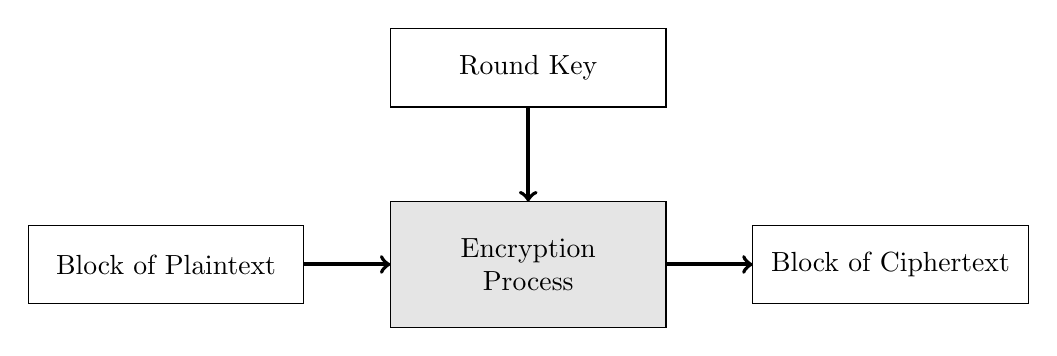
\begin{tikzpicture}
        \node at (4.6, 2.5) [rectangle, draw, align=center, minimum width=3.5cm, minimum height=1cm] {Round Key};
        \node at (4.6, 0) [rectangle, draw, fill=black!10, align=center, text width = 2cm, minimum width=3.5cm, minimum height=1.6cm] {Encryption Process};
        \node at (0, 0) [rectangle, draw, align=center, minimum width=3.5cm, minimum height=1cm] {Block of Plaintext};
        \node at (9.2, 0) [rectangle, draw, align=center, minimum width=3.5cm, minimum height=1cm] {Block of Ciphertext};
        \draw[->, line width=0.5mm] (1.75, 0) -- (2.85, 0);
        \draw[->, line width=0.5mm] (4.6+1.75, 0) -- (4.6+1.75+1.1, 0);
        \draw[->, line width=0.5mm] (4.6, 2) -- (4.6, 0.8);
    \end{tikzpicture}
    \caption{A diagram of the basic flow of a block cipher.}
\end{figure}

Though there are different types of block ciphers, most are referred to as \textit{iterated block ciphers} \cite{wiki:block_cipher}. 
In an iterated block cipher, for every block of plaintext, the cipher produces an identically sized block of ciphertext. Each iteration of the cipher is 
known as a \textit{round} \cite{wiki:block_cipher}. In each round, the blocks are operated on via a reversible transformation function 
known as a \textit{round function} \cite{wiki:block_cipher}.

The round function will also typically take in different \textit{round keys} as a secondary input. These round keys are created from the original key. 

\begin{align*}
    \mathlarger{M_i = R_{K_i}(M_{i-1})}
\end{align*}

The equation above defines the generic operation of a round where $M_0$ represents the plaintext and $M_r$ represents the ciphertext, where 
$r$ represents the number of rounds.

\begin{align*}
    \mathlarger{M_0\;} & \mathlarger{= M \oplus K_0} \\
    \mathlarger{M_i\;} & \mathlarger{= R_{K_i}(M_{i - 1});\; i=1 \ldots r} \\
    \mathlarger{C\;} & \mathlarger{= M_r \oplus K_{r + 1}} \\
\end{align*}

\subsection{Feistel Cipher}

A \textit{Feistel cipher} (also commonly referred to as \textit{Feistel network}) is a cryptographic model used for creating block ciphers \cite{wiki:feistel_cipher}.
In a Feistel cipher, a block is split into two equal-sized halves. The round function is then applied to one half, which is then XORed with the other half \cite{wiki:feistel_cipher}. 
The resulting halves are then swapped with each other \cite{wiki:feistel_cipher}.

The basic encryption process for a Feistel cipher where $F(K, R)$ represents the round function and $K_0,K_1,\ldots,K_n$ represents the subkeys for the rounds 
$0,1,\ldots,n$ respectively---are as follows:

\begin{enumerate}
    \item Split the plaintext into two equal halves, $L_0$ and $R_0$, respectively.
    \item For each round $i = 0,1,\ldots,n$ where $n$ represents the amount of rounds, compute the following: 
        \begin{align*}
            \mathlarger{L_{i + 1}\;} & \mathlarger{= R_i} \\
            \mathlarger{R_{i + 1}\;} & \mathlarger{= L_i \oplus F(R_i,K_i)}
        \end{align*}
            
        where $F(K,R)$ represents the round function.
\end{enumerate}

The resulting block of ciphertext is then $(L_{n + 1},R_{n + 1})$.

The process to decrypt a block of ciphertext is the reverse of the encryption process. For each round $i = n,n-1,\ldots,0$ where $n$ represents the amount of rounds, 
we compute the following:
\begin{align*}
    \mathlarger{R_{i}\;} & \mathlarger{= L_i+1} \\
    \mathlarger{L_{i}\;} & \mathlarger{= R_i+1 \oplus F(L_i+1,K_i)}
\end{align*}

Once again, the resulting block of plaintext is then $(L_0,R_0)$.

\begin{figure}[H]
    \centering
    \begin{tikzpicture}
        \definecolor{greenarrow}{RGB}{0,120,10}
        \definecolor{redarrow}{RGB}{120,0,0}
        \node at (1, 6) {Plaintext};
        \node at (0, 5.4) [rectangle, draw, fill=blue!10, align=center, minimum width=2cm, minimum height=0.4cm] {$L_0$};
        \node at (2, 5.4) [rectangle, draw, fill=blue!10, align=center, minimum width=2cm, minimum height=0.4cm] {$R_0$};
         
        \draw[fill=purple!10] (1, 4.5) ellipse (0.5cm and 0.3cm);
        \node at (1, 4.5) {$K_0$};
        \node at (1, 3.5) [rectangle, draw, fill=yellow!10, align=center, minimum width=0.5cm, minimum height=0.5cm] {F};
        \draw[->] (1, 4.2) -- (1, 3.75);
        \draw (0, 3.5) circle (0.2cm);
        \draw (0, 3.7) -- (0, 3.3);
        \draw (-0.2, 3.5) -- (0.2, 3.5);
        \draw[->] (0.75, 3.5) -- (0.2, 3.5);
        \draw[->] (2, 3.5) -- (1.25, 3.5);
         
        \draw[fill=purple!10] (1, 2) ellipse (0.5cm and 0.3cm);
        \node at (1, 2) {$K_1$};
        \node at (1, 1) [rectangle, draw, fill=yellow!10, align=center, minimum width=0.5cm, minimum height=0.5cm] {F};
        \draw[->] (1, 1.7) -- (1, 1.25);
        \draw (0, 1) circle (0.2cm);
        \draw (0, 1.2) -- (0, 0.8);
        \draw (-0.2, 1) -- (0.2, 1);
        \draw[->] (0.75, 1) -- (0.2, 1);
        \draw[->] (2, 1) -- (1.25, 1);
         
        \newcommand{\down}{3}
        \draw[fill=purple!10] (1, 2-\down) ellipse (0.5cm and 0.3cm);
        \node at (1, 2-\down) {$K_n$};
        \node at (1, 1-\down) [rectangle, draw, fill=yellow!10, align=center, minimum width=0.5cm, minimum height=0.5cm] {F};
        \draw[->] (1, 1.7-\down) -- (1, 1.25-\down);
        \draw (0, 1-\down) circle (0.2cm);
        \draw (0, 1.2-\down) -- (0, 0.8-\down);
        \draw (-0.2, 1-\down) -- (0.2, 1-\down);
        \draw[->] (0.75, 1-\down) -- (0.2, 1-\down);
        \draw[->] (2, 1-\down) -- (1.25, 1-\down);
         
        \draw[->, draw=greenarrow, thick] (0, 5.15) -- (0, 3.7);
        \draw[draw=greenarrow, thick] (0, 3.3) -- (0, 3.1) -- (2, 2.9) -- (2, 0.6) -- (0, 0.4);
        \draw[->, draw=redarrow, thick] (2, 5.15) -- (2, 3.1) -- (0, 2.9) -- (0, 1.2);
        \draw[draw=redarrow, thick] (0, 0.8) -- (0, 0.6) -- (2, 0.4);
        \draw[->, draw=greenarrow, thick] (0, 0) -- (0, -1.8);
        \draw[->, draw=greenarrow, thick] (0, -2.2) -- (0, -2.5);
        \draw[->, draw=redarrow, thick] (2, 0) -- (2, -2.5);
         
        \node at (0, -2.8) [rectangle, draw, fill=blue!10, align=center, minimum width=2cm, minimum height=0.4cm] {$R_{n+1}$};
        \node at (2, -2.8) [rectangle, draw, fill=blue!10, align=center, minimum width=2cm, minimum height=0.4cm] {$L_{n+1}$};
        \node at (1, -3.5) {Ciphertext};
         
        \draw[thick,dashed] (1, 0.2) -- (1, -0.4);
         
        \begin{scope}[xshift=6cm]
        \node at (1, 6) {Ciphertext};
        \node at (0, 5.4) [rectangle, draw, fill=blue!10, align=center, minimum width=2cm, minimum height=0.4cm] {$R_{n+1}$};
        \node at (2, 5.4) [rectangle, draw, fill=blue!10, align=center, minimum width=2cm, minimum height=0.4cm] {$L_{n+1}$};
         
        \draw[fill=purple!10] (1, 4.5) ellipse (0.5cm and 0.3cm);
        \node at (1, 4.5) {$K_n$};
        \node at (1, 3.5) [rectangle, draw, fill=yellow!10, align=center, minimum width=0.5cm, minimum height=0.5cm] {F};
        \draw[->] (1, 4.2) -- (1, 3.75);
        \draw (0, 3.5) circle (0.2cm);
        \draw (0, 3.7) -- (0, 3.3);
        \draw (-0.2, 3.5) -- (0.2, 3.5);
        \draw[->] (0.75, 3.5) -- (0.2, 3.5);
        \draw[->] (2, 3.5) -- (1.25, 3.5);
         
        \draw[fill=purple!10] (1, 2) ellipse (0.5cm and 0.3cm);
        \node at (1, 2) {$K_{n-1}$};
        \node at (1, 1) [rectangle, draw, fill=yellow!10, align=center, minimum width=0.5cm, minimum height=0.5cm] {F};
        \draw[->] (1, 1.7) -- (1, 1.25);
        \draw (0, 1) circle (0.2cm);
        \draw (0, 1.2) -- (0, 0.8);
        \draw (-0.2, 1) -- (0.2, 1);
        \draw[->] (0.75, 1) -- (0.2, 1);
        \draw[->] (2, 1) -- (1.25, 1);
         
        \draw[fill=purple!10] (1, 2-\down) ellipse (0.5cm and 0.3cm);
        \node at (1, 2-\down) {$K_0$};
        \node at (1, 1-\down) [rectangle, draw, fill=yellow!10, align=center, minimum width=0.5cm, minimum height=0.5cm] {F};
        \draw[->] (1, 1.7-\down) -- (1, 1.25-\down);
        \draw (0, 1-\down) circle (0.2cm);
        \draw (0, 1.2-\down) -- (0, 0.8-\down);
        \draw (-0.2, 1-\down) -- (0.2, 1-\down);
        \draw[->] (0.75, 1-\down) -- (0.2, 1-\down);
        \draw[->] (2, 1-\down) -- (1.25, 1-\down);
         
        \draw[->, draw=redarrow, thick] (0, 5.15) -- (0, 3.7);
        \draw[draw=redarrow, thick] (0, 3.3) -- (0, 3.1) -- (2, 2.9) -- (2, 0.6) -- (0, 0.4);
        \draw[->, draw=greenarrow, thick] (2, 5.15) -- (2, 3.1) -- (0, 2.9) -- (0, 1.2);
        \draw[draw=greenarrow, thick] (0, 0.8) -- (0, 0.6) -- (2, 0.4);
        \draw[->, draw=redarrow, thick] (0, 0) -- (0, -1.8);
        \draw[->, draw=redarrow, thick] (0, -2.2) -- (0, -2.5);
        \draw[->, draw=greenarrow, thick] (2, 0) -- (2, -2.5);
         
        \node at (0, -2.8) [rectangle, draw, fill=blue!10, align=center, minimum width=2cm, minimum height=0.4cm] {$L_0$};
        \node at (2, -2.8) [rectangle, draw, fill=blue!10, align=center, minimum width=2cm, minimum height=0.4cm] {$R_0$};
        \node at (1, -3.5) {Plaintext};
         
        \draw[thick,dashed] (1, 0.2) -- (1, -0.4);
        \end{scope}
    \end{tikzpicture}
    \caption{A diagram depicting the encryption and decryption process in a Feistel cipher.}
\end{figure}

\subsubsection{Data Encryption Standard}

The \textit{Data Encryption Standard} (or \textit{DES} for short) is a symmetric-key algorithm. The algorithm was developed in the early 1970s by IBM and is based
off the design of the Feistel cipher. The algorithm (after a few changes) was eventually published as an official United States \textit{Federal Information Processing 
Standard} (or \textit{FIPS} for short) in 1977. The publication of the algorithm resulted in international adoption and academic critic \cite{wiki:des}. 

The Data Encryption Standard is now generally regarded to as insecure (for many applications) \cite{wiki:des}. This is mainly because DES has a relatively small key size of 
56 bits. Despite this, DES was "highly influential in the advancements of modern cryptography." \cite{wiki:des} 

DES is structured much like any other iterated block cipher. In the cipher, a block consists of 64-bits \cite{wiki:des}. Also, DES uses a key to modify the 
transformational operations---a key is effectively only 56-bits as the algorithm uses 8-bits for error checking (and thus disregarding them in the actual operations) 
\cite{wiki:des}.

DES additionally makes use of \textit{initial} and \textit{final} permutations. Before transforming a block, an initial permutation table is applied to the 64-bit block of data.
Once the block is operated on, a final permutation table is applied to the resulting 64-bit block of data. The initial permutation table reverses the actions of the
final permutation table, and vice-versa \cite{wiki:des}.

\begin{figure}[H]
    \centering
    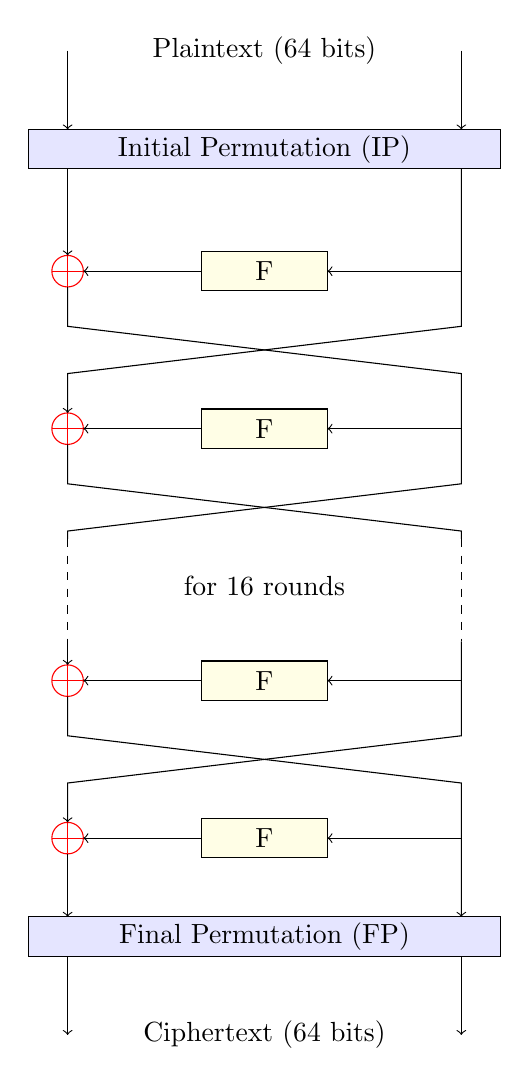
\begin{tikzpicture}
        \node at (3, 11) {Plaintext (64 bits)};
        \draw[fill=blue!10] (0, 10) rectangle (6, 9.5);
        \node at (3, 9.75) {Initial Permutation (IP)};
        \begin{scope}[yshift=8.2cm]
        \draw[fill=yellow!10] (2.2, 0.25) rectangle (3.8, -0.25);
        \node at (3, 0) {F};
        \draw[draw=red] (0.5, 0) circle [radius=0.2];
        \draw[draw=red] (0.3, 0) -- (0.7, 0);
        \draw[draw=red] (0.5, 0.2) -- (0.5, -0.2);
        \draw[->] (5.5, 0) -- (3.8, 0);
        \draw[->] (2.2, 0) -- (0.7, 0);
        \end{scope}
        \begin{scope}[yshift=6.2cm]
        \draw[fill=yellow!10] (2.2, 0.25) rectangle (3.8, -0.25);
        \node at (3, 0) {F};
        \draw[draw=red] (0.5, 0) circle [radius=0.2];
        \draw[draw=red] (0.3, 0) -- (0.7, 0);
        \draw[draw=red] (0.5, 0.2) -- (0.5, -0.2);
        \draw[->] (5.5, 0) -- (3.8, 0);
        \draw[->] (2.2, 0) -- (0.7, 0);
        \end{scope}
        \begin{scope}[yshift=3.0cm]
        \draw[fill=yellow!10] (2.2, 0.25) rectangle (3.8, -0.25);
        \node at (3, 0) {F};
        \draw[draw=red] (0.5, 0) circle [radius=0.2];
        \draw[draw=red] (0.3, 0) -- (0.7, 0);
        \draw[draw=red] (0.5, 0.2) -- (0.5, -0.2);
        \draw[->] (5.5, 0) -- (3.8, 0);
        \draw[->] (2.2, 0) -- (0.7, 0);
        \end{scope}
        \begin{scope}[yshift=1.0cm]
        \draw[fill=yellow!10] (2.2, 0.25) rectangle (3.8, -0.25);
        \node at (3, 0) {F};
        \draw[draw=red] (0.5, 0) circle [radius=0.2];
        \draw[draw=red] (0.3, 0) -- (0.7, 0);
        \draw[draw=red] (0.5, 0.2) -- (0.5, -0.2);
        \draw[->] (5.5, 0) -- (3.8, 0);
        \draw[->] (2.2, 0) -- (0.7, 0);
        \end{scope}
        \draw[fill=blue!10] (0, 0) rectangle (6, -0.5);
        \node at (3, -0.25) {Final Permutation (FP)};
        \node at (3, -1.5) {Ciphertext (64 bits)};
         
        \draw[->] (0.5, 11) -- (0.5, 10);
        \draw[->] (5.5, 11) -- (5.5, 10);
         
        \draw[->] (0.5, 9.5) -- (0.5, 8.4);
        \draw (0.5, 8) -- (0.5, 7.5) -- (5.5, 6.9) -- (5.5, 5.5) -- (0.5, 4.9) -- (0.5, 4.8);
        \draw[dashed] (0.5, 4.8) -- (0.5, 3.5);
        \draw[->] (0.5, 3.5) -- (0.5, 3.2);
        \draw[->] (0.5, 2.8) -- (0.5, 2.3) -- (5.5, 1.7) -- (5.5, 0);
         
        \draw[->] (5.5, 9.5) -- (5.5, 7.5) -- (0.5, 6.9) -- (0.5, 6.4);
        \draw (0.5, 6) -- (0.5, 5.5) -- (5.5, 4.9) -- (5.5, 4.8);
        \draw[dashed] (5.5, 4.8) -- (5.5, 3.5);
        \draw[->] (5.5, 3.5) -- (5.5, 2.3) -- (0.5, 1.7) -- (0.5, 1.2);
        \draw[->] (0.5, 0.8) -- (0.5, 0);
         
        \draw[->] (0.5, -0.5) -- (0.5, -1.5);
        \draw[->] (5.5, -0.5) -- (5.5, -1.5);
         
        \node at (3, 4.2) {for 16 rounds};
    \end{tikzpicture}
    \caption{The overall structure of DES.}
\end{figure}

In each round, a \textit{subkey} derived from the original key is used to transform the block of data (the subkeys are supplied in the reverse order when decrypting).
The subkeys are produced from a table known as the \textit{key schedule}. The key schedule defines how the original key should be rotated to create a subkey from a given
round. A \textit{permutation choice 1} (or \textit{PC1} for short) table is applied onto the original key before the subkey process. For each subkey, a \textit{permutation
choice 2} (or \textit{PC2} for short) table is applied.

\begin{figure}[H]
    \centering
    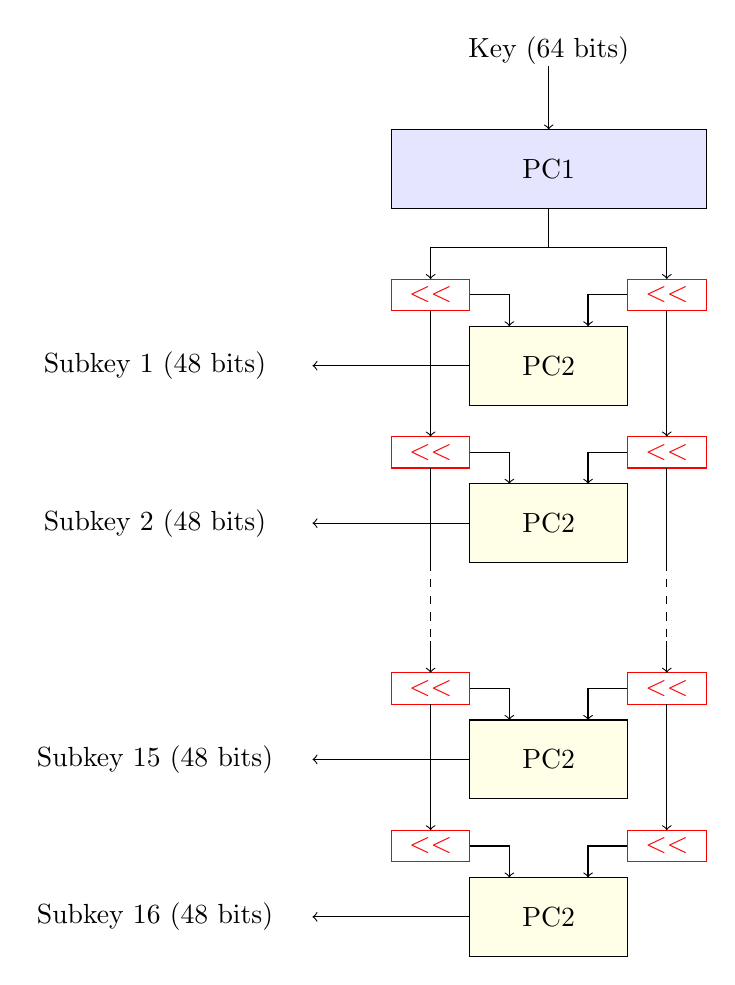
\begin{tikzpicture}
        \node at (6, 10) {Key (64 bits)};
        \draw[fill=blue!10] (4, 9) rectangle (8, 8);
        \node at (6, 8.5) {PC1};
        \draw[->] (6, 9.8) -- (6, 9);
         
        \begin{scope}[yshift=6cm]
        \draw[fill=yellow!10] (5, 0.5) rectangle (7, -0.5);
        \node at (6, 0) {PC2};
        \draw[draw=red] (4, 1.1) rectangle (5, 0.7);
        \node at (4.5, 0.9) {\textcolor{red}{$<<$}};
        \draw[draw=red] (7, 1.1) rectangle (8, 0.7);
        \node at (7.5, 0.9) {\textcolor{red}{$<<$}};
        \draw[->] (5, 0.9) -- (5.5, 0.9) -- (5.5, 0.5);
        \draw[->] (7, 0.9) -- (6.5, 0.9) -- (6.5, 0.5);
        \draw[->] (5, 0) -- (3, 0);
        \end{scope}
        \begin{scope}[yshift=4cm]
        \draw[fill=yellow!10] (5, 0.5) rectangle (7, -0.5);
        \node at (6, 0) {PC2};
        \draw[draw=red] (4, 1.1) rectangle (5, 0.7);
        \node at (4.5, 0.9) {\textcolor{red}{$<<$}};
        \draw[draw=red] (7, 1.1) rectangle (8, 0.7);
        \node at (7.5, 0.9) {\textcolor{red}{$<<$}};
        \draw[->] (5, 0.9) -- (5.5, 0.9) -- (5.5, 0.5);
        \draw[->] (7, 0.9) -- (6.5, 0.9) -- (6.5, 0.5);
        \draw[->] (5, 0) -- (3, 0);
        \end{scope}
        \begin{scope}[yshift=1cm]
        \draw[fill=yellow!10] (5, 0.5) rectangle (7, -0.5);
        \node at (6, 0) {PC2};
        \draw[draw=red] (4, 1.1) rectangle (5, 0.7);
        \node at (4.5, 0.9) {\textcolor{red}{$<<$}};
        \draw[draw=red] (7, 1.1) rectangle (8, 0.7);
        \node at (7.5, 0.9) {\textcolor{red}{$<<$}};
        \draw[->] (5, 0.9) -- (5.5, 0.9) -- (5.5, 0.5);
        \draw[->] (7, 0.9) -- (6.5, 0.9) -- (6.5, 0.5);
        \draw[->] (5, 0) -- (3, 0);
        \end{scope}
        \begin{scope}[yshift=-1cm]
        \draw[fill=yellow!10] (5, 0.5) rectangle (7, -0.5);
        \node at (6, 0) {PC2};
        \draw[draw=red] (4, 1.1) rectangle (5, 0.7);
        \node at (4.5, 0.9) {\textcolor{red}{$<<$}};
        \draw[draw=red] (7, 1.1) rectangle (8, 0.7);
        \node at (7.5, 0.9) {\textcolor{red}{$<<$}};
        \draw[->] (5, 0.9) -- (5.5, 0.9) -- (5.5, 0.5);
        \draw[->] (7, 0.9) -- (6.5, 0.9) -- (6.5, 0.5);
        \draw[->] (5, 0) -- (3, 0);
        \end{scope}
         
        \draw (6, 8) -- (6, 7.5);
        \draw[->] (6, 7.5) -- (4.5, 7.5) -- (4.5, 7.1);
        \draw[->] (6, 7.5) -- (7.5, 7.5) -- (7.5, 7.1);
        \draw[->] (4.5, 6.7) -- (4.5, 5.1);
        \draw[->] (7.5, 6.7) -- (7.5, 5.1);
        \draw (4.5, 4.7) -- (4.5, 3.5);
        \draw[dashed] (4.5, 3.5) -- (4.5, 2.5);
        \draw[->] (4.5, 2.5) -- (4.5, 2.1);
        \draw (7.5, 4.7) -- (7.5, 3.5);
        \draw[dashed] (7.5, 3.5) -- (7.5, 2.5);
        \draw[->] (7.5, 2.5) -- (7.5, 2.1);
        \draw[->] (4.5, 1.7) -- (4.5, 0.1);
        \draw[->] (7.5, 1.7) -- (7.5, 0.1);
         
        \node at (1, 6) {Subkey 1 (48 bits)};
        \node at (1, 4) {Subkey 2 (48 bits)};
        \node at (1, 1) {Subkey 15 (48 bits)};
        \node at (1, -1) {Subkey 16 (48 bits)};
    \end{tikzpicture}
    \caption{The structure of the DES key schedule. The $\mathsmaller{<<}$ denotes a rotation to the left.}
\end{figure}

The round $F(K, R)$ function is defined as follows:

\begin{enumerate}
    \item The 32-bit half-block is expanded to 48-bits using the \textit{expansion permutation table} (E). The expansion permutation duplicates half of the bits in the 
          32-bit block in order to expand the data. 
    \item The result of the expansion is then combined with the given subkey for the round (using a XOR operation).
    \item The result of the key combination is split into eight 6-bit blocks of data which is then processed by the \textit{substitution boxes}---one 6-bit block for 
    each substitution-box. Each substitution-box replaces the 6-bit input data with a 4-bit output. The substitution values are non-linearly transformed.
    \item Lastly, the outputs from the substitution process are combined into one 32-bit block of data which is rearranged by a fixed permutation table known as the
        \textit{permutation-box}. The permutation-box shuffles the output of each substitution to increase cryptographic security.
\end{enumerate}

\begin{figure}[H]
    \centering
    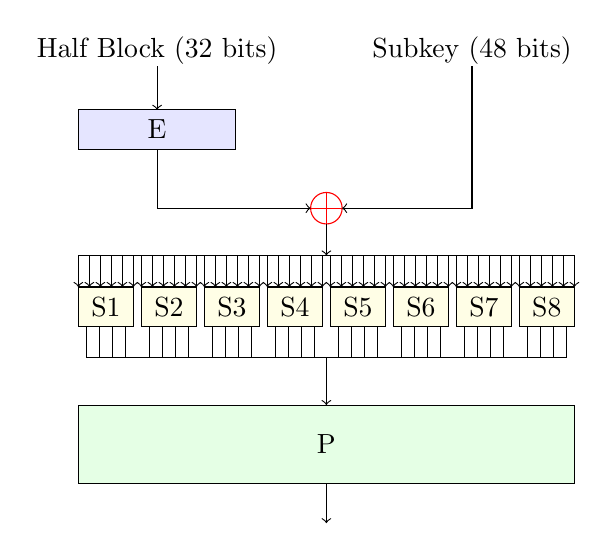
\begin{tikzpicture}
        \node at (1, 6) {Half Block (32 bits)};
        \node at (5, 6) {Subkey (48 bits)};
        \draw[fill=blue!10] (0, 5.25) rectangle (2, 4.75);
        \node at (1, 5) {E};
        \draw[draw=red] (3.15, 4) circle [radius=0.2];
        \draw[draw=red] (2.95, 4) -- (3.35, 4);
        \draw[draw=red] (3.15, 4.2) -- (3.15, 3.8);
        \draw[->] (1, 5.8) -- (1, 5.25);
        \draw[->] (1, 4.75) -- (1, 4) -- (2.95, 4);
        \draw[->] (5, 5.8) -- (5, 4) -- (3.35, 4);
        \draw[->] (3.15, 3.8) -- (3.15, 3.4);
        \draw (0, 3.4) -- (6.3, 3.4);
        \begin{scope}[xshift=0cm]
        \draw[fill=yellow!10] (0, 3) rectangle (0.7, 2.5);
        \node at (0.35, 2.75) {S1};
        \draw[->] (0, 3.4) -- (0, 3);
        \draw[->] (0.14, 3.4) -- (0.14, 3);
        \draw[->] (0.28, 3.4) -- (0.28, 3);
        \draw[->] (0.42, 3.4) -- (0.42, 3);
        \draw[->] (0.56, 3.4) -- (0.56, 3);
        \draw[->] (0.7, 3.4) -- (0.7, 3);
        \draw (0.1, 2.5) -- (0.1, 2.1);
        \draw (0.267, 2.5) -- (0.267, 2.1);
        \draw (0.433, 2.5) -- (0.433, 2.1);
        \draw (0.6, 2.5) -- (0.6, 2.1);
        \end{scope}
        \begin{scope}[xshift=0.8cm]
        \draw[fill=yellow!10] (0, 3) rectangle (0.7, 2.5);
        \node at (0.35, 2.75) {S2};
        \draw[->] (0, 3.4) -- (0, 3);
        \draw[->] (0.14, 3.4) -- (0.14, 3);
        \draw[->] (0.28, 3.4) -- (0.28, 3);
        \draw[->] (0.42, 3.4) -- (0.42, 3);
        \draw[->] (0.56, 3.4) -- (0.56, 3);
        \draw[->] (0.7, 3.4) -- (0.7, 3);
        \draw (0.1, 2.5) -- (0.1, 2.1);
        \draw (0.267, 2.5) -- (0.267, 2.1);
        \draw (0.433, 2.5) -- (0.433, 2.1);
        \draw (0.6, 2.5) -- (0.6, 2.1);
        \end{scope}
        \begin{scope}[xshift=1.6cm]
        \draw[fill=yellow!10] (0, 3) rectangle (0.7, 2.5);
        \node at (0.35, 2.75) {S3};
        \draw[->] (0, 3.4) -- (0, 3);
        \draw[->] (0.14, 3.4) -- (0.14, 3);
        \draw[->] (0.28, 3.4) -- (0.28, 3);
        \draw[->] (0.42, 3.4) -- (0.42, 3);
        \draw[->] (0.56, 3.4) -- (0.56, 3);
        \draw[->] (0.7, 3.4) -- (0.7, 3);
        \draw (0.1, 2.5) -- (0.1, 2.1);
        \draw (0.267, 2.5) -- (0.267, 2.1);
        \draw (0.433, 2.5) -- (0.433, 2.1);
        \draw (0.6, 2.5) -- (0.6, 2.1);
        \end{scope}
        \begin{scope}[xshift=2.4cm]
        \draw[fill=yellow!10] (0, 3) rectangle (0.7, 2.5);
        \node at (0.35, 2.75) {S4};
        \draw[->] (0, 3.4) -- (0, 3);
        \draw[->] (0.14, 3.4) -- (0.14, 3);
        \draw[->] (0.28, 3.4) -- (0.28, 3);
        \draw[->] (0.42, 3.4) -- (0.42, 3);
        \draw[->] (0.56, 3.4) -- (0.56, 3);
        \draw[->] (0.7, 3.4) -- (0.7, 3);
        \draw (0.1, 2.5) -- (0.1, 2.1);
        \draw (0.267, 2.5) -- (0.267, 2.1);
        \draw (0.433, 2.5) -- (0.433, 2.1);
        \draw (0.6, 2.5) -- (0.6, 2.1);
        \end{scope}
        \begin{scope}[xshift=3.2cm]
        \draw[fill=yellow!10] (0, 3) rectangle (0.7, 2.5);
        \node at (0.35, 2.75) {S5};
        \draw[->] (0, 3.4) -- (0, 3);
        \draw[->] (0.14, 3.4) -- (0.14, 3);
        \draw[->] (0.28, 3.4) -- (0.28, 3);
        \draw[->] (0.42, 3.4) -- (0.42, 3);
        \draw[->] (0.56, 3.4) -- (0.56, 3);
        \draw[->] (0.7, 3.4) -- (0.7, 3);
        \draw (0.1, 2.5) -- (0.1, 2.1);
        \draw (0.267, 2.5) -- (0.267, 2.1);
        \draw (0.433, 2.5) -- (0.433, 2.1);
        \draw (0.6, 2.5) -- (0.6, 2.1);
        \end{scope}
        \begin{scope}[xshift=4cm]
        \draw[fill=yellow!10] (0, 3) rectangle (0.7, 2.5);
        \node at (0.35, 2.75) {S6};
        \draw[->] (0, 3.4) -- (0, 3);
        \draw[->] (0.14, 3.4) -- (0.14, 3);
        \draw[->] (0.28, 3.4) -- (0.28, 3);
        \draw[->] (0.42, 3.4) -- (0.42, 3);
        \draw[->] (0.56, 3.4) -- (0.56, 3);
        \draw[->] (0.7, 3.4) -- (0.7, 3);
        \draw (0.1, 2.5) -- (0.1, 2.1);
        \draw (0.267, 2.5) -- (0.267, 2.1);
        \draw (0.433, 2.5) -- (0.433, 2.1);
        \draw (0.6, 2.5) -- (0.6, 2.1);
        \end{scope}
        \begin{scope}[xshift=4.8cm]
        \draw[fill=yellow!10] (0, 3) rectangle (0.7, 2.5);
        \node at (0.35, 2.75) {S7};
        \draw[->] (0, 3.4) -- (0, 3);
        \draw[->] (0.14, 3.4) -- (0.14, 3);
        \draw[->] (0.28, 3.4) -- (0.28, 3);
        \draw[->] (0.42, 3.4) -- (0.42, 3);
        \draw[->] (0.56, 3.4) -- (0.56, 3);
        \draw[->] (0.7, 3.4) -- (0.7, 3);
        \draw (0.1, 2.5) -- (0.1, 2.1);
        \draw (0.267, 2.5) -- (0.267, 2.1);
        \draw (0.433, 2.5) -- (0.433, 2.1);
        \draw (0.6, 2.5) -- (0.6, 2.1);
        \end{scope}
        \begin{scope}[xshift=5.6cm]
        \draw[fill=yellow!10] (0, 3) rectangle (0.7, 2.5);
        \node at (0.35, 2.75) {S8};
        \draw[->] (0, 3.4) -- (0, 3);
        \draw[->] (0.14, 3.4) -- (0.14, 3);
        \draw[->] (0.28, 3.4) -- (0.28, 3);
        \draw[->] (0.42, 3.4) -- (0.42, 3);
        \draw[->] (0.56, 3.4) -- (0.56, 3);
        \draw[->] (0.7, 3.4) -- (0.7, 3);
        \draw (0.1, 2.5) -- (0.1, 2.1);
        \draw (0.267, 2.5) -- (0.267, 2.1);
        \draw (0.433, 2.5) -- (0.433, 2.1);
        \draw (0.6, 2.5) -- (0.6, 2.1);
        \end{scope}
        \draw (0.1, 2.1) -- (6.2, 2.1);
        \draw[->] (3.15, 2.1) -- (3.15, 1.5);
        \draw[fill=green!10] (0, 1.5) rectangle (6.3, 0.5);
        \node at (3.15, 1) {P};
        \draw[->] (3.15, 0.5) -- (3.15, 0);
    \end{tikzpicture}
    \caption{The structure of the round function in DES. \textit{S1-S8} denote their respective substitution box.}
\end{figure}